\subsection{Rhytmus}
Rhythmus ist einer der fundamentalen Aspekte der Musiktheorie. Um gute Harmonien und Melodien komponieren zu können, musst du verstehen, wie Rhythmus funktioniert und wie du ihn in deinen Tracks einsetzt. Anhand von Rhythmus wird Musik systematisch in Taktschläge bzw. Beats eingeteilt, die sich innerhalb eines Taktes mit einem allgemein anerkannten Tempo wiederholen. Noten, Melodien und Akkorde kann man leicht als Vibrationen in der Luft definieren, die von unserem Trommelfell wahrgenommen werden.

\textbf{Hier  eventuell Takt erklaeren}

Rhythmus hingegen hat eher etwas mit der einzigartigen Wahrnehmung von Zeit zu tun, über die der Mensch verfügt. Zumindest ist das die Definition, die dir ein Metronom geben würde. Rhythmus ist etwas, dass mit der einzigartigen Wahrnehmung von Zeit zu tun, über die der Mensch verfügt. Um Rhythmus zu verstehen, muss man vier grundlegende Konzepte kennen:

\begin{itemize}
    \item \textbf{Taktschläge (=Beats) und Noten}
    \item \textbf{Takte und Taktangaben}
    \item \textbf{Schwache (=unbetonte) und starke (=betonte) Zählzeiten}
    \item \textbf{Zweier- und Dreiertakte}
\end{itemize}

Wenn du diese vier Grundkonzepte beherrschst, kannst du besser üben und neue, interessante Rhythmen in deinen Tracks verwenden. Um zum Zentrum eines Rhythmus vorzudringen, musst du verstehen, dass eine Musiknote die zeitliche Dauer, während der ein Instrument gespielt wird, repräsentiert. 

\subsubsection{Taktschläge und Noten}
Eine ganze Note ist die längste Tondauer, doch ganze Noten können in halbe, Viertel-, Achtel- und Sechzehntelnoten runtergebrochen werden.

\begin{table}[H]
    \caption{Taktschläge und Noten}
    \begin{tabularx}{\textwidth}{| X | X | X |}
    \hline
    Note & Pause & Anschlag Pro Takt \\ \hline
    \Ganz & \GaPa  & 1 \\ \hline
    \Halb & \HaPa & 2 \\ \hline
    \Vier & \ViPa  & 4 \\ \hline
    \Acht & \AcPa  & 8 \\ \hline
    \Sech & \SePa & 16 \\ \hline
    \end{tabularx}
\end{table}

Es gibt vieles, dem man sich widmen muss, wenn man verstehen will, wie man musikalische Rhythmen liest.Doch um zum Zentrum eines Rhythmus vorzudringen, musst du verstehen, dass eine Musiknote die zeitliche Dauer, während der ein Instrument gespielt wird, repräsentiert. Eine ganze Note ist die längste Tondauer, doch ganze Noten können in halbe, Viertel-, Achtel- und Sechzehntelnoten runtergebrochen werden. Eine halbe Note nimmt lediglich die halbe Dauer einer ganzen Note in Anspruch, eine Viertelnote ein Viertel.


\subsubsection{Takte und Taktangaben}
Jeder Musik liegt ein Puls zugrunde, der in bestimmte Zeiteinheiten gefasst werden kann. Diese Zeiteinheit werden als Takte bezeichnet. In der westlichen Musik geben die Taktangaben eines Songs vor, wie sein Puls in jedem Takt gemessen wird, und das Tempo legt fest, wie schnell der Puls ist. Nehmen wir die gängigste Taktart in der Musik – den 4/4-Takt.
Die obere Vier gibt an, dass es vier Taktschläge in einem Takt gibt, und die untere Vier gibt an, dass alle Taktschläge in Viertelnoten gemessen werden.

\begin{figure}[H]
    \centering
    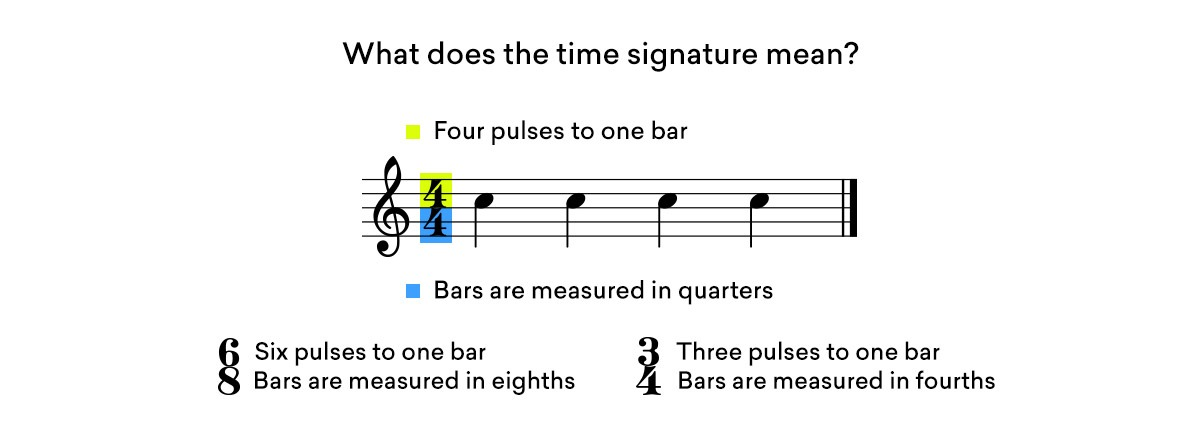
\includegraphics[width=0.8\textwidth]{images/Rythm_body}
\end{figure}

Natürlich gibt es noch viel mehr Taktarten als den 4/4-Takt. Alle Walzer sind im ¾-Takt und dann gibt es auch noch die Geschichte mit zusammengesetzten und ungeraden Taktarten.

\subsubsection{Starke und schwache Zählzeiten}
Ok, jetzt da du weißt, wie Taktarten funktionieren und Taktschläge in einen Takt passen, sollten wir uns anschauen, wie Rhythmus innerhalb eines Taktes funktioniert. Innerhalb eines Taktes gibt es starke Taktschläge, die den Puls vorantreibenund schwache Taktschläge,die dem Puls entgegenwirken. Im 4/4-Takt zum Beispiel fallen die starken Taktschläge auf die erste und dritte Viertelnote im Takt, und die schwachen Taktschläge fallen auf die zweite und vierte Viertelnote.

\begin{figure}[H]
    \centering
    
\includegraphics[width=0.8\textwidth]{images/Rythm_body_2}
\end{figure}

Im ¾-Takt fällt der starke Taktschlag auf die erste Viertelnote und die schwachen Taktschläge fallen auf die zweite und dritte Viertelnote.

\begin{figure}[H]
    \centering
    
\includegraphics[width=0.8\textwidth]{images/Rythm_body_3}
\end{figure}

Wenn du dich erstmal mit starken und schwachen Taktschlägen beschäftigt hast, hörst du sie überall. Beispiele dafür sind der EINS-zwei, EINS-zwei Puls einer Kick-Drum in einem 4/4-Disco-Song oder das EINS-zwei-drei, EINS-zwei-drei eines Walzers.

\subsubsection{Zweier- und Dreiertakte}
Bisher haben wir uns nur mit dem ¾- und 4/4-Takt, den beiden gängigsten Taktarten, beschäftigt. Falls du zusammengesetzte und ungerade Taktarten in deinem Track verwenden willst, musst du verstehen, dass Taktschläge innerhalb eines Taktes in Zweier- und Dreierpaaren gefühlt werden. Das Ganze macht mehr Sinn, wenn du weißt, wie starke und schwache Taktschläge funktionieren. Eine Art, Dreier- und Zweiertakte zu visualisieren, besteht darin, sich den Unterschied zwischen einem rollenden Dreieck und einem rollenden Quadrat vorzustellen, bei dem mit jeder neuen Umdrehung ein starker Taktschlag fällt.

Wenn du dir die starken und schwachen Taktschläge in einem 4/4-Takt anschaust, kannst du sie in zwei Zweier-gruppen unterteilen – stark – schwach, stark – schwach.

\begin{figure}[H]
    \centering
    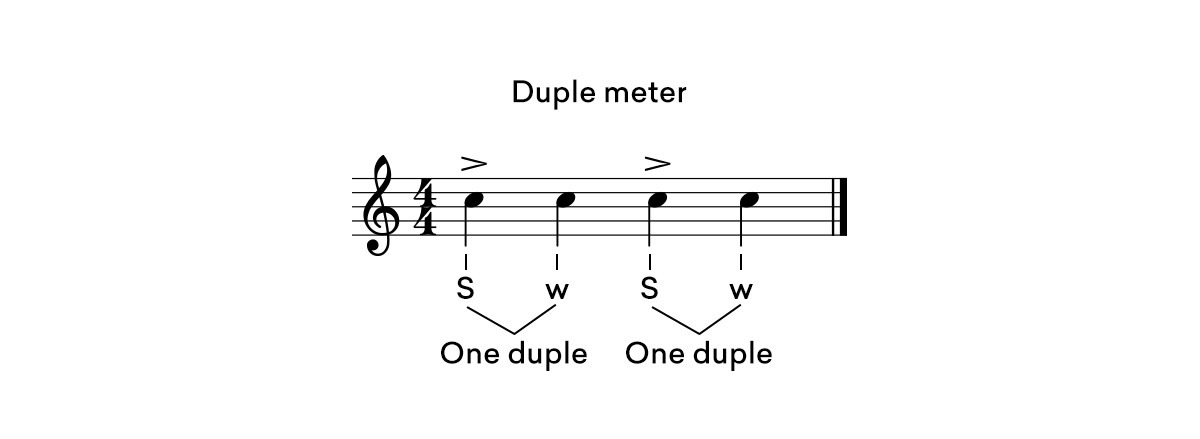
\includegraphics[width=0.8\textwidth]{images/Rythm_body_4}
\end{figure}

Ein stark-schwach-Muster bedeutet, dass es sich um einen Zweiertakt handelt. Da er in zwei Zweierpaare unterteilt ist, wird der 4/4-Takt manchmal auch Quadrupel-Takt genannt. Im ¾-Takt gibt es nur eine Dreiergruppe – stark – schwach – schwach.

\begin{figure}[H]
    \centering
    
\includegraphics[width=0.8\textwidth]{images/Rythm_body_5}
\end{figure}

Ein stark-schwach-schwach-Muster bedeutet, dass es sich um einen Dreiertakt handelt. Jedes rhythmische Muster und jeder Takt kann in Zweier- oder Dreiermetren unterteilt werden.

\subsubsection{Simple vs. zusammengesetzte Taktarten}
Simple und zusammengesetzte Taktarten hängen direkt mit dem Metrum zusammen. Das Metrum legt fest, wie der Rhythmus anhand von starken und schwachen Taktschlägen gefühlt wird. Simple und zusammengesetzte Taktarten bestimmen, ob eine Einheit aus kürzeren Noten (meistens Achtelnoten) in Zweier- oder Dreiergruppen aufgeteilt wird. Simple Taktarten gruppieren Achtelnoten in Zweiergruppen. Der 4/4-Takt ist ein simpler Zweiertakt. Seine Achtelnoten werden gezählt als EINS-und, zwei-und, DREI-und, vier-und.

\begin{figure}[H]
    \centering
    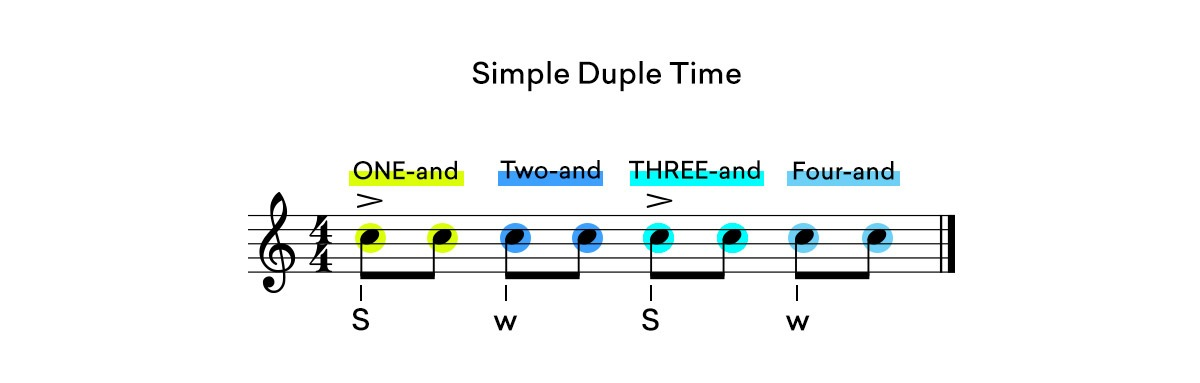
\includegraphics[width=0.8\textwidth]{images/Rythm_body_6}
\end{figure}

Der ¾-Takt ist ein simpler Dreiertakt. Er wird gezählt als EINS-und, zwei-und, drei-und.

\begin{figure}[H]
    \centering
    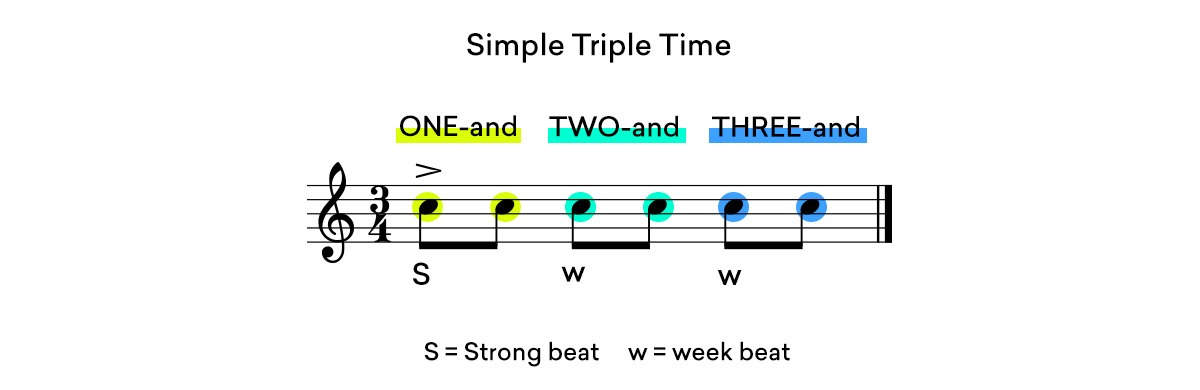
\includegraphics[width=0.8\textwidth]{images/Rythm_body_7}
\end{figure}

Zusammengesetzte Taktarten gruppieren Achtelnoten in Dreiergruppen. 6/8 und 9/8 sind beide Beispiele für eine zusammengesetzte Taktart. Im zusammengesetzten 6/8-Zweiertakt werden die Noten in zwei Gruppen aus jeweils drei Achtelnoten unterteilt.

\begin{figure}[H]
    \centering
    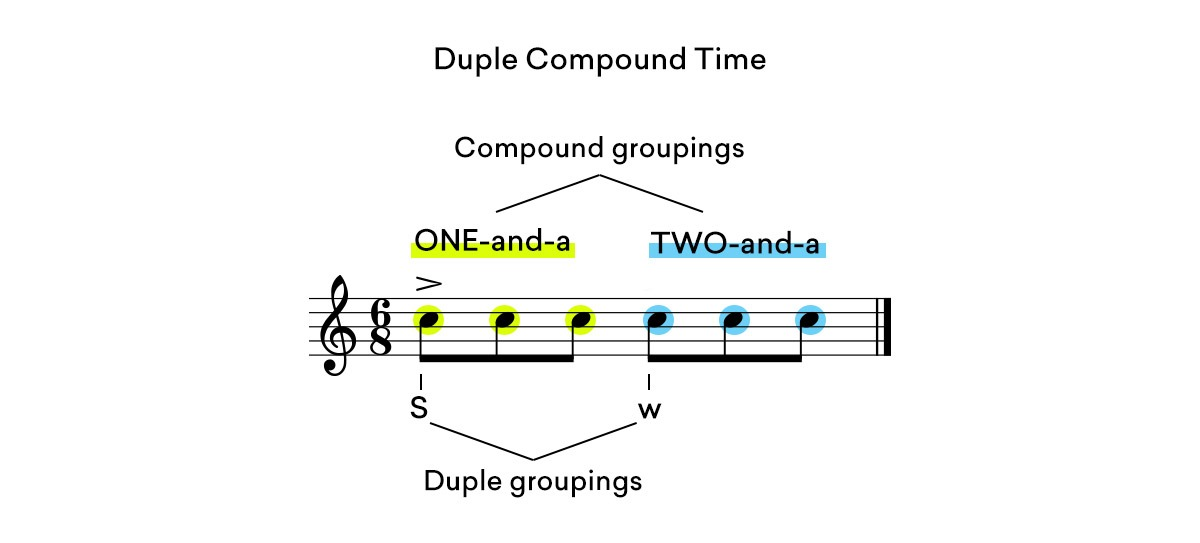
\includegraphics[width=0.8\textwidth]{images/Rythm_body_8}
\end{figure}

Die Achtelnoten könnten somit als EINS-und-a, ZWEI-und-a gezählt werden. Drakes Song Plastic Bag ist ein tolles Beispiel für einen Pop-Song, der dem 6/8-Rhythmus folgt. Im zusammengesetzten 9/8-Dreiertakt sind die Noten in drei Gruppen aus drei Achtelnoten unterteilt.

\begin{figure}[H]
    \centering
    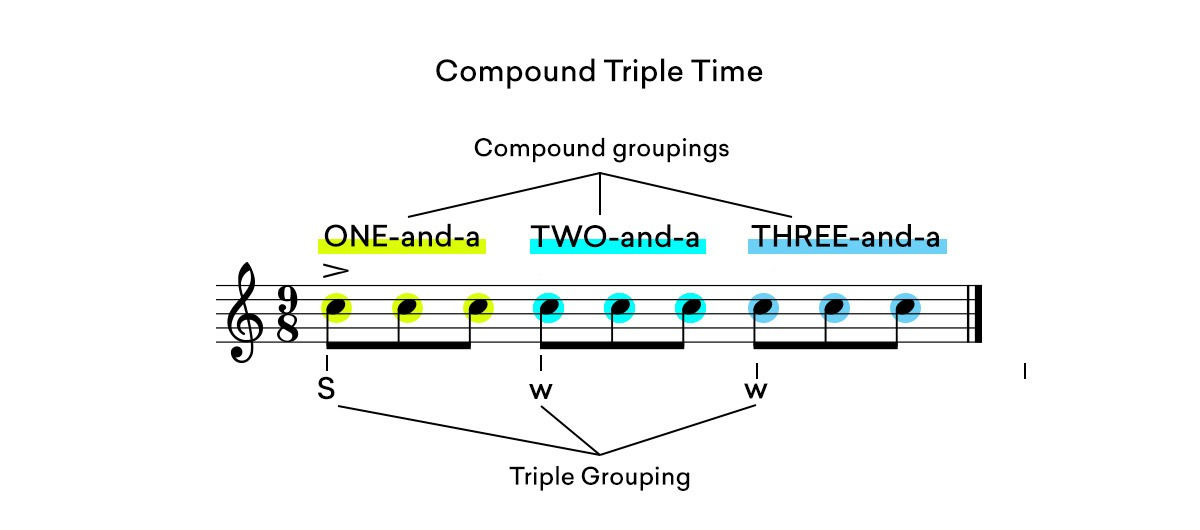
\includegraphics[width=0.8\textwidth]{images/Rythm_body_9}
\end{figure}

Die Achtelnoten werden gezählt als EINS-und-a, ZWEI-und-a, DREI-und-a. Der berühmte Jazz-Track Blue Rondo A La Turk von Dave Brubeck ist ein gutes Beispiel für den 9/8-Takt. Der Rhythmus in diesem Track wechselt zwischen dem zusammengesetzten und ungeraden 9/8-Takt. Finde heraus, ob den den Unterschied hören kannst!

\subsubsection{Ungerade Taktarten}
Ungerade Takte können etwas einschüchternd sein, es gibt viel zu wissen auf diesem Gebiet. Doch wenn du erstmal weißt, wie Zweier- und Dreiermetren funktionieren, kommst du auch mit jedem ungeraden Takt klar. Ungerade Taktarten gehen noch viel weiter mit den Regeln als simple und zusammengesetzte Taktarten, indem sie sie kombinieren. Das liegt daran, dass alle ungeraden Taktarten einem Muster folgen, das auf einer Kombination aus Zweier- und Dreiergruppen basiert. Schauen wir uns den 5{/8}-Takt an. Er kann entweder aus einer Zweiergruppe plus einer Dreiergruppe bestehen, oder einer Dreiergruppe plus einer Zweiergruppe.

\begin{figure}[H]
    \centering
    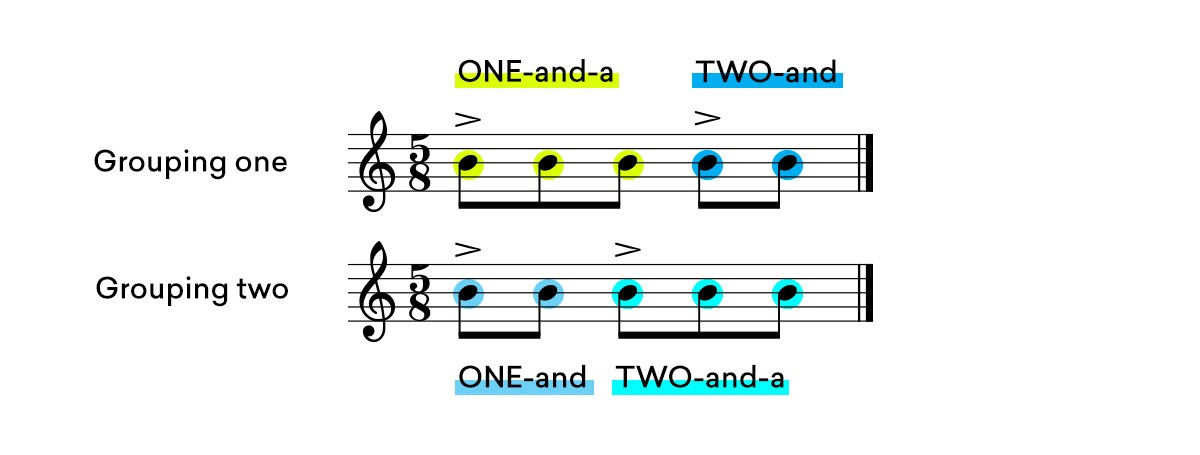
\includegraphics[width=0.8\textwidth]{images/Rythm_body_10}
\end{figure}

Falls das deiner Meinung nach keinen Sinn ergibt, versuche es einfach damit, das Metrum laut mitzuzählen, jedoch nur in Dreier- und Zweiergruppen. Für einen  5/8-Takt würdest du dementsprechend entweder EINS-und ZWEI-und-a zählen, oder EINS-und-a ZWEI-und. Wenn wir uns wieder Blue Rondo A La Turk als Beispiel ansehen, dann folgt der 9/8-Teil als ungerader Takt dem Muster EINS-und, ZWEI-und, DREI-und, VIER-und-a.

\begin{figure}[H]
    \centering
    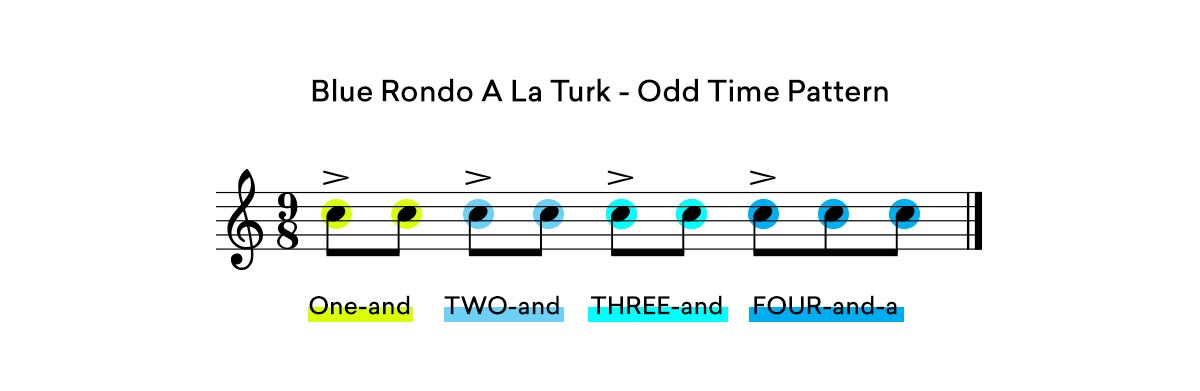
\includegraphics[width=0.8\textwidth]{images/Rythm_body_11}
\end{figure}